\section{Discrete Fourier Transform Basics}

\begin{enumerate}[label=\alph*), leftmargin=*]
%% a)
\item
%
The Fourier Transform (FT) of a sine wave at $f_{0}=20Hz$ is discrete, since the time series is periodic, comprising of Dirac $\delta$ functions at $\pm f_{0}$,
provided at figure \ref{fig:1_1_a}. Since the windowing (multiplication) operation in time domain is equivalent to convolution in the frequency domain,
the Discrete Time Fourier Transform (DTFT) of a windowed sine wave at $20Hz$ is derived by convolution of the ideal FT of the sine wave,
Dirac $\delta$ functions, with the FT of the rectangular window, $sinc$ function, illustrated at figure \ref{fig:1_1_a} for different window lengths $\tau$.
The spectrum leakage is demonstrated, as well as the trade-off between side-lobes peak and window length $\tau$ (inverse relationship).
%
\begin{figure}[h]
    \centering
    \begin{subfigure}{0.49\textwidth}
        \centering
        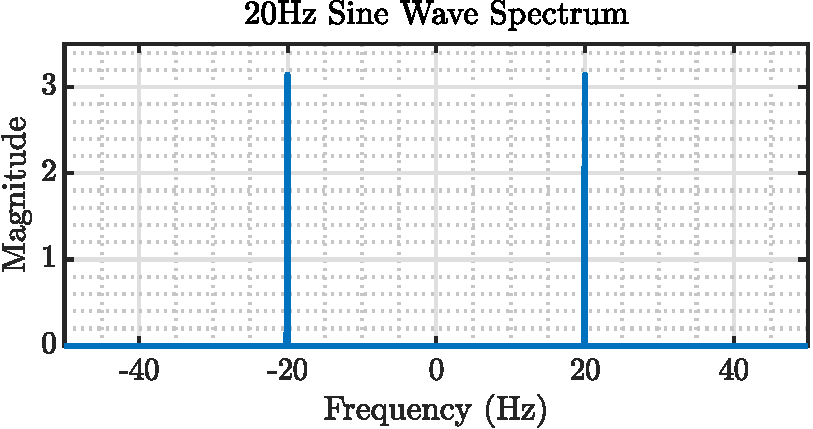
\includegraphics[height=1.5in]{report/spectrum-estimation/discete-fourier-transform-basics/assets/a/sine-ideal-spectrum}
    \end{subfigure}
    ~ 
    \begin{subfigure}{0.49\textwidth}
        \centering
        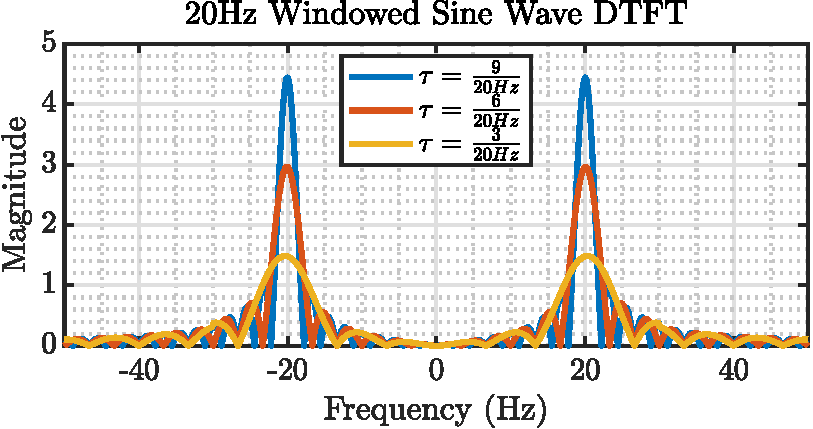
\includegraphics[height=1.5in]{report/spectrum-estimation/discete-fourier-transform-basics/assets/a/dtft-theoretical-window}
    \end{subfigure}
    \caption{Ideal magnitude spectrum (left) and theoretical DTFT (right) of $20Hz$ sine wave.}
    \label{fig:1_1_a}
\end{figure}


%% b)
\item
%
The Discrete Fourier Transform (DFT) spectrum of a finite length sine wave at $f_{0}=20Hz$ is considered. The signal can be treated as
a windowed and sampled version of the continuous, infinite length sine wave. Consequently, its DFT is expected to be a sampled version of the DTFT shown
in figure \ref{fig:1_1_a}, at frequency intervals defined by the frequency resolution $\Delta f = \frac{F_{s}}{K}$, where $F_{s}$ and $K$ the sampling frequency
and the sequence length, respectively. In case of $K=100$, we obtain $F_{s}=1000Hz$ and $\Delta f = 10Hz$, leading to elimination of spectrum leakage or
\textbf{coherent sampling}, since at the integer multiples of the frequency resolution $10Hz$, the $sinc$ function is zero, excluding the peaks at $\pm f_{0}$.
We highlight that this is not the same with the ideal FT spectrum, but just the result of frequency quantisation. If $f_{0}$ or $F_{s}$ are slightly perturbed
then the leakage will be inevitable. When zero-padding is performed and $K=1000$, then $\Delta f = 1Hz$ and the impact of the spectrum leakage is evident.
Figure \ref{fig:1_1_b} illustrated the DFT spectra of those experiments.
%
\begin{figure}[H]
    \centering
    \begin{subfigure}{0.49\textwidth}
        \centering
        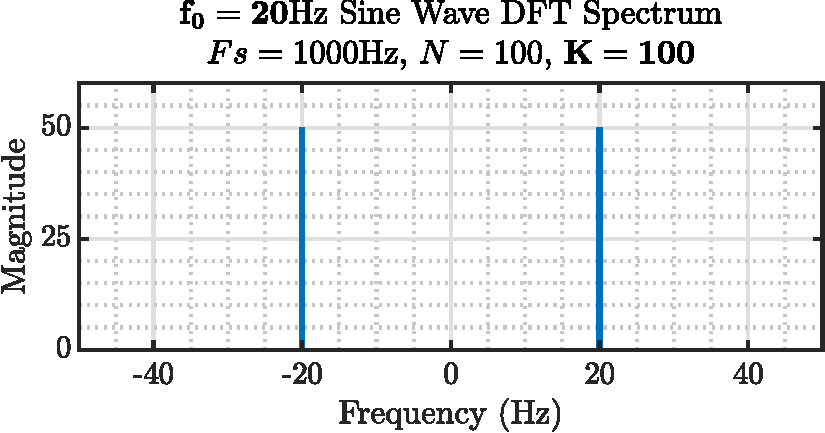
\includegraphics[height=1.5in]{report/spectrum-estimation/discete-fourier-transform-basics/assets/b/dft-f0_20-K_100}
    \end{subfigure}
    ~ 
    \begin{subfigure}{0.49\textwidth}
        \centering
        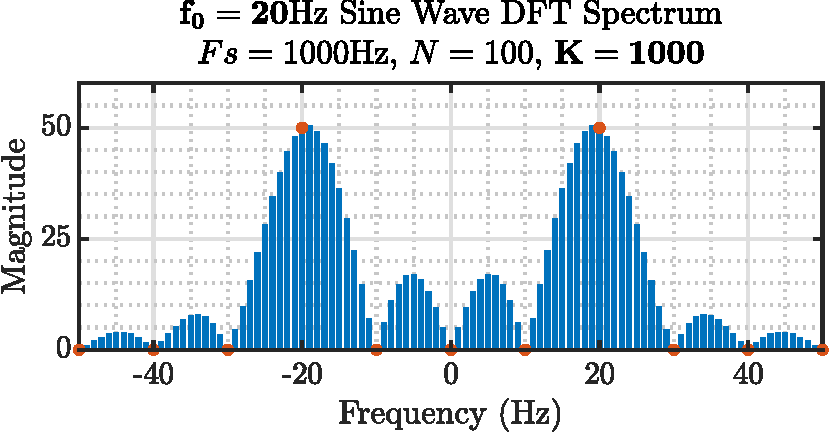
\includegraphics[height=1.5in]{report/spectrum-estimation/discete-fourier-transform-basics/assets/b/dft-f0_20-K_1000}
    \end{subfigure}
    \caption{$20Hz$ sampled sine wave DFT spectra and coherent sampling.}
    \label{fig:1_1_b}
\end{figure}


%% c)
\item
%
The experiment is repeated for a finite length sine wave at $f_{1}=24Hz$ and its spectra are provided at \ref{fig:1_1_c}.
As expected this time for both $K=100$ and $K=1000$ spectral leakage is unavoidable. However, especially in case of $K=100$
when $\Delta f = 10Hz$, we note that the peaks at $\pm f_{1} = \pm 24Hz$ are undetected and therefore the sequence is
incoherently sampled. Increasing the zero-padding samples, such that the frequency resolution $\Delta f$ is a factor of $f_{1}$
resolves this issue, therefore nothing can be done for the spectral leakage effect. Candidate values for $K$ then are:
$125, \frac{1000}{6}, 250, 500, 1000, \cdots$.
%
\begin{figure}[H]
    \centering
    \begin{subfigure}{0.49\textwidth}
        \centering
        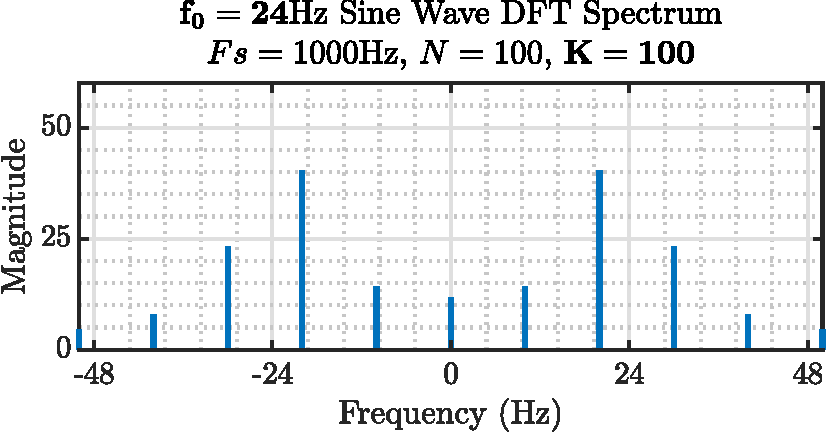
\includegraphics[height=1.5in]{report/spectrum-estimation/discete-fourier-transform-basics/assets/c/dft-f0_24-K_100}
    \end{subfigure}
    ~ 
    \begin{subfigure}{0.49\textwidth}
        \centering
        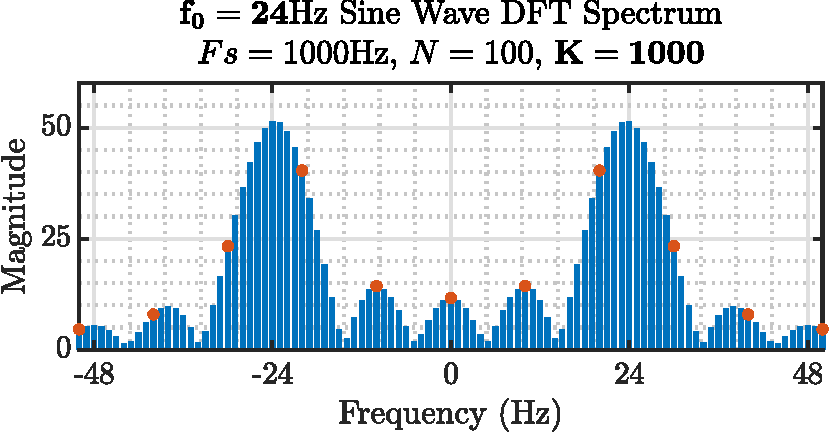
\includegraphics[height=1.5in]{report/spectrum-estimation/discete-fourier-transform-basics/assets/c/dft-f0_24-K_1000}
    \end{subfigure}
    \caption{$24Hz$ sampled sine wave DFT spectra and incoherent sampling.}
    \label{fig:1_1_c}
\end{figure}
\end{enumerate}